\documentclass[12pt]{article}
\usepackage[T1]{fontenc} % Added to support Bold Small Caps font shapes

% \usepackage{authblk}
\usepackage{color}
% \usepackage[all]{xy}
\usepackage{subcaption}
\usepackage{amsmath,epsfig}
\usepackage{amssymb,amsthm}
\usepackage{setspace}
\usepackage{float}
%\usepackage{cite}

% Changed linkcolor=black to remove blue text/outlines in TOC, while keeping citations blue
\usepackage[colorlinks=true, linkcolor=black, citecolor=blue, urlcolor=blue, breaklinks=true]{hyperref}

% ── TOC Formatting Package ──
% Moved ABOVE parskip to prevent the "\@starttoc has already been redefined" warning
\usepackage{tocloft} 

% ── Packages added for GitHub reference sheet ──
\usepackage{listings}
\usepackage{xcolor}
\usepackage{enumitem}
\usepackage{parskip}
\usepackage{courier}
\usepackage{titlesec}

% ── Code block styling (used in gitHub.tex) ──
\lstset{
    basicstyle=\ttfamily\small,
    backgroundcolor=\color{gray!10},
    frame=single,
    framerule=0.4pt,
    rulecolor=\color{gray!50},
    breaklines=true,
    xleftmargin=8pt,
    xrightmargin=8pt,
    aboveskip=6pt,
    belowskip=6pt
}

% ── Section styling ──
%\titleformat{\section}{\large\bfseries}{}{0em}{}[\titlerule]
%\titleformat{\subsection}{\normalsize\bfseries}{}{0em}{}

\newcommand{\R}{\mathcal{R}}

% =====================================================================
% CITATION SETUP: Custom BibLaTeX (Mimics Springer Math Bio Style)
% =====================================================================
\usepackage[
    backend=biber, 
    style=authoryear, 
    maxcitenames=2, 
    maxbibnames=99, 
    giveninits=true, 
    terseinits=true, 
    uniquename=init, % Added to fix the biblatex conflicting options warning
    dashed=false, 
    url=false, 
    doi=true
]{biblatex}

% Remove quotation marks from article titles
\DeclareFieldFormat[article,inbook,incollection,inproceedings,patent,thesis,unpublished]{title}{#1}

% Remove the word "In:" before journal names
\renewbibmacro{in:}{%
  \ifentrytype{article}{}{\printtext{\bibstring{in}\intitlepunct}}}

% Remove "pp." from page numbers in articles
\DeclareFieldFormat[article]{pages}{#1}

% Format Volume and Number as Volume:Number
\renewbibmacro*{volume+number+eid}{%
  \printfield{volume}%
  \setunit*{\addcolon}%
  \printfield{number}%
  \setunit{\addcomma\space}%
  \printfield{eid}}

\addbibresource{References.bib}
% =====================================================================

\usepackage[margin=1.0in]{geometry}
\usepackage{graphicx}

% =====================================================================
% TABLE OF CONTENTS SETUP
% =====================================================================
% 1. Center the "Contents" title and make it Small Caps
\renewcommand{\cfttoctitlefont}{\hfill\Large\scshape\bfseries}
\renewcommand{\cftaftertoctitle}{\hfill\mbox{}}

% 2. Add dotted lines to Sections (the article class hides these by default)
\renewcommand{\cftsecleader}{\cftdotfill{\cftdotsep}}

% 3. Make Section titles and Section page numbers bold
\renewcommand{\cftsecfont}{\bfseries}
\renewcommand{\cftsecpagefont}{\bfseries}

\begin{document}

% =====================================================================
% CUSTOM TITLE PAGE
% =====================================================================
\begin{titlepage}
    \begin{center}
    \vspace*{1cm}
    \line(1,0){450} \\
    [.25in]
    \huge{\bfseries Reaction Diffusion Model for a Waterborne Pathogen} \\
    [2mm]
    \line(1,0){400} \\
    [1.5cm]
    \textsc{\LARGE University of Tennessee at Chattanooga}\\
    [.5cm]
    %\textsc{\Large PhD in Computational Science: Applied Mathematics} \\
    
    \vfill % Pushes the bottom block down automatically
    
    \textsc{\Large Advisor: Dr. Jin Wang} \\
    \textsc{\small UTC Department of Mathematics} \\
    [1cm]
    \textsc{\Large Ethan Reyes} \\
    \textsc{\small qww165@mocs.utc.edu} \\
    [1cm]
    \textsc{\Large July 2026}
    \vspace*{1cm}
    \end{center}
\end{titlepage}

% =====================================================================
% ABSTRACT PLACEHOLDER
% =====================================================================
\begin{abstract}
    TBD
    \\
    \\ \textbf{Keywords:} \emph{Reaction-Diffusion, Waterborne Pathogen, Numerical Simulation, Cholera}
\end{abstract}

\newpage

% =====================================================================
% TABLE OF CONTENTS
% =====================================================================
\pagenumbering{roman}
\tableofcontents
\newpage
\pagenumbering{arabic}

% =====================================================================
% MAIN CONTENT
% =====================================================================
% !TEX root = main.tex
\newpage 
\section{Introduction}

\noindent
{\large A reaction-diffusion model for waterborne infection}

\vskip0.2in
We consider a waterborne disease, such as cholera, that can be transmitted 
from both the environment-to-human and human-to-human pathways.
As a starting point, we consider a one-dimensional (1D) spatial domain
$ 0 \leq x \leq a$ for some positive constant $a$
which may represent a river containing the pathogen.

Let the population densities of the susceptible, infected, and recovered individuals be
$S(x, t)$, $I(x, t)$, and $R(x,t)$ respectively, at location $x$ and time $t$.
Let also the pathogen concentration in the river be $B(x,t)$. 
We have the following reaction-diffusion equations to describe 
the disease transmission:
\begin{equation}
\begin{aligned}
 & \frac{\partial S}{\partial t} - c_1 \frac{\partial^2 S}{\partial x^2} 
   = \Lambda - \alpha SB - \beta SI - \mu S, \\
 & \frac{\partial I}{\partial t} - c_2 \frac{\partial^2 I}{\partial x^2} 
   =  \alpha SB + \beta SI - (\mu + \omega + \gamma) I, \\
 & \frac{\partial R}{\partial t} - c_3 \frac{\partial^2 R}{\partial x^2}   
   =  \gamma I-\mu R , \\
 &  \frac{\partial B}{\partial t} + v \frac{\partial B}{\partial x} 
   - d \frac{\partial^2 B}{\partial x^2} = g B \big(1 - \frac{B}{K} \big) +\xi I - \delta B,   
\end{aligned} 
 \label{eqn-recdiff}
\end{equation}
for $ 0 < x < L$ and $ t > 0$.
The parameters $c_1$, $c_2$ and $c_3$ are the diffusion rates of the susceptible,
infected, and recovered individuals,
respectively;
$\Lambda$ is the population influx rate, $\alpha$ is the environment-to-human 
transmission rate,
$\beta$ is the human-to-human transmission rate,
$\mu$ is the natural death rate, $\omega$ is the disease-induced death rate, and
$\gamma$ is the disease recovery rate.
In addition, $g$ is the intrinsic growth rate of the waterborne pathogen,
$K$ is its carrying capacity, $\xi$ is the shedding rate of infected hosts,
$\delta$ is the removal rate of the pathogen from the aquatic environment, 
$d$ is the pathogen diffusion rate, 
and $v$ is the pathogen advection rate that represents the speed of the river flow.


We may use no-flux boundary conditions for system \eqref{eqn-recdiff}:
\begin{equation}
\begin{aligned}
&  \frac{\partial Y}{\partial x}(0, t) = 0, \quad 
  \frac{\partial Y}{\partial x}(L, t) = 0, \quad {\rm where} \;\; Y = S, I, R; \\
& v B(0, t) - d \frac{\partial B}{\partial x}(0, t) = 0 , \quad
 v B(L, t) - d \frac{\partial B}{\partial x}(L, t) = 0, 
\end{aligned}
 \label{bc-noflux}
\end{equation}
for $ t >0$.
Meanwhile, we need to provide appropriate initial conditions:
\begin{equation}
  Y(x,0) = Y_0(x) \geq 0, \quad {\rm where} \;\; Y = S, I, R, B, 
 \label{ic-host}
\end{equation}
for $0 \leq x \leq L$.






% !TEX root = main.tex
\section{Numerical Simulations}
\subsection{Biological Parameters \& Initialization}

In this section we define and explain the different biological parameters used in the simulation. To start, the simulated length of the river is assumed to have length $3\pi$ expressed as $0 \leq x \leq 3 \pi$. Since the temporal domain is chose to be from $t = 0$ to $t = 12$ each variable must be adjusted to be monthly rates. For example, the average human lifespan of a human in the simulation is assumed to be 43.5 years (\cite{wu_threshold_2024}), which expressed as months would be $\mu = \frac{1}{43.5*12} = 0.0019$. Similar conversions follow for the other parameters used and displayed in the table below. 
\begin{table}[H]
\centering
\caption{Biological interpretations and values for model parameters}
%Parameter values were adapted from the framework used in \cite{wang_reaction-advection-diffusion_2022} and were slightly adjusted or modified to suit the purposes of this paper. Values marked with an asterisk ($^*$) are estimated for these specific simulations.
\label{tab:parameters}
\renewcommand{\arraystretch}{1.3} 
\begin{tabular}{llc}
\hline
\textbf{Parameter} & \textbf{Description} & \textbf{Value} \\ \hline
$\Lambda$ & Influx rate of susceptible humans & $19.0$ \\
$\alpha$ & Base indirect contact rate (environment-to-human) & $0.00033$ \\
$\beta$ & Base direct contact rate (human-to-human) & $0.00047$ \\
$\mu$ & Natural death rate of human hosts & $0.0019$ \\
$\omega$ & Disease-induced death rate & varied \\
$\gamma$ & Recovery rate of infectious hosts & $6.0$ \\
$\delta$ & Natural death rate of Cholera in water & $1.0$ \\
$\xi$ & Base shedding rate of Cholera by infectious humans & $300$ \\
$g_0$ & Baseline intrinsic growth rate of Cholera & $0.5$ \\
$g_1$ & Seasonal fluctuation amplitude of Cholera growth & $0.5$ \\
$K$ & Maximal capacity of free-living Cholera in water & 200,000 \\
$c_1$ & Diffusion coefficient of susceptible humans & $1.0$ \\
$c_2$ & Diffusion coefficient of infectious humans & $0.5$ \\
$c_3$ & Diffusion coefficient of recovered humans & $0.8$ \\
$d$ & Diffusion coefficient of Cholera in the water & $0.1$ \\
$v$ & Advection coefficient of Cholera (river flow) & varied \\ \hline
%$c$ & Relative rate of bacterial loss at downstream & $2.0$ \\ \hline
\end{tabular}
\end{table}
The 
The parameters chosen for our simulation were inspired by the framework and criteria used in papers by \cite{wang_reaction-advection-diffusion_2022} and \cite{wu_threshold_2024}. The parameters $\omega$ and $v$ were tested at different values during the experiment. In particular we let $\omega = 0$ or $\omega  = .001$ for our experiments. With an estimated $21,000$ to $143,000$ deaths out of the 1.3 to 4.0 million cases \cite{who_cholera_2025}, it is reasonable to test these particular values. Furthermore, for advection coefficient of Cholera (river flow) we tested the following values: 
$v \in \{ 0, \, 0.1, \, 0.7, \, 1.2\}$. Each of the tested values was chosen to represent stagnant water, slow, moderate, and fast flow respectively. 
%\newpage %-=


Since the temporal domain of the simulation is a full year, $0 \leq t \leq 12$, we introduce a seasonality function to realistically model the seasonal osculations due to climate events. Furthermore, we apply the rates of $\alpha, \beta, \xi, $ and $g$ to function function used to properly simulate seasonality and spatial heterogeneity.  

\begin{align*}
    \alpha_{t_n} &= \alpha  \, \cdot \, H(x)T(t_n) \\
    \beta_{t_n} &= \beta  \, \cdot \, H(x)T(t_n) \\ 
    \xi_{t_n} &= \xi  \, \cdot \, H(x)T(t_n) \\
\end{align*}
Where the spatial heterogeneity is represented by $H(x) = \frac{1}{2} - \frac{1}{4} \cos(2x)$ and our seasonality function is defined as $T(t_n) =\frac{1}{2} - \frac{1}{4} \sin\big(\frac{2 \pi t_n}{12}\big) $. The spatial heterogeneity function forces the model to simulate different clusters of humans along the river where these clustered would equivalent to villages in the real world. These functions created the spatial heterogeneity needed but are not as robust as other functions used to for an adaptive human behavior approach found as found in other research papers such as \cite{wang2015influence}. Next we present the effective growth rate of Cholera:
\begin{equation*}
    g_{t_n} = g_0 + g_1 \sin\big(\frac{\pi \cdot t_n}{6}\big)
\end{equation*}
In our model, $g$ represents the intrinsic growth rate of the waterborne pathogen. However, since the growth rate of Cholera varies in different temperatures (\cite{constantin_de_magny_cholera_2009}) we use a periodic function. Since our temporal domain is $0 \leq t \leq 12$, we let our periodic function be $\sin\big(\frac{\pi \cdot t_n}{6}\big)$ so that it completes one full cycle exactly at the end of our domain. 
Finally we present the initial conditions used in our simulation: 
\begin{align}
    S^0_{i} &=  \frac{\Lambda}{\mu} - 500 \cos(2x)\\
    I^0_{i} &=  1 - \cos(2x)\\
    R^0_{i} &=  0\\
    B^0_{i} &=  .5 - .3 \cos(2x)\\
\end{align}
To start, the susceptible initial condition used was chosen to again account for spatial heterogeneity throughout the simulated length of the river. In other words, this simulates different pockets or clusters of susceptible individuals along the river. We translate the three full cycles of $\cos(2x)$ on its domain $0 \leq x \leq 3\pi$ to simulate three distinct locations of infection at $t = 0$ which will then be moved downward with advection. Since, we are $t=0$ we naturally assume there to be 0 recovered individuals to start. Next, we use the same $\cos(2x)$ to simulated slightly more concentration of the pathogen in the water where infected individuals are located. 
\subsection{Numerical Scheme}
We discretize the spatial domain $[0, L]$ into $N_x$ uniformly spaced nodes, where each node is defined by $x_i = i \Delta x$ for $i = 0, 1, \dots, N_x-1$. Similarly, the temporal domain $[0, T]$ is discretized into $N_t$ time steps defined by $t_n = n \Delta t$ for $n = 0, 1, \dots, N_t-1$. Let $U_i^n$ denote the numerical approximation of a state variable at location $x_i$ and time $t_n$. Now that the spatial and temporal domains are discretized we introduce the general form of a forward time and central space finite difference method. 
\begin{equation*}
    w_i^{n+1} = w_i^n + \frac{c \Delta t}{\Delta x^2} \left[  w_{i+1}^n - 2w_i^n + w_{i-1}^n  \right]
\end{equation*}
Before we apply this method to our system we first simplify the reaction terms of each equation. Note that that the pathogen includes a first order spatial derivative which we will also approximate using central difference formula.
\begin{align}
    F_S(S, I, B) &= \Lambda - \alpha S B - \beta S I - \mu S \\[6pt]
    F_I(S, I, B) &= \alpha S B + \beta S I - (\mu + \omega + \gamma) I \\[6pt]
    F_R(I, R) &= \gamma I - \mu R \\[6pt]
    F_B(B, I) &= g B \left(1 - \frac{B}{K}\right) + \xi I - \delta B
\end{align}
After condensing the reaction terms we can now apply the general FTCS method to our system of equation which yields the new following system for the interior spatial nodes ($0 < i < N_x - 1$):
\begin{align}
    S_i^{n+1} &= S_i^n + \Delta t \left[ c_1 \frac{S_{i+1}^n - 2S_i^n + S_{i-1}^n}{(\Delta x)^2} + F_S(S_i^n, I_i^n, B_i^n) \right] \label{susceptible} \\[10pt]
    I_i^{n+1} &= I_i^n + \Delta t \left[ c_2 \frac{I_{i+1}^n - 2I_i^n + I_{i-1}^n}{(\Delta x)^2} + F_I(S_i^n, I_i^n, B_i^n) \right] \label{infected} \\[10pt]
    R_i^{n+1} &= R_i^n + \Delta t \left[ c_3 \frac{R_{i+1}^n - 2R_i^n + R_{i-1}^n}{(\Delta x)^2} + F_R(I_i^n, R_i^n) \right] \label{recovered} \\[10pt]
    B_i^{n+1} &= B_i^n + \Delta t \left[ d \frac{B_{i+1}^n - 2B_i^n + B_{i-1}^n}{(\Delta x)^2} - v \frac{B_{i+1}^n - B_{i-1}^n}{2\Delta x} + F_B(B_i^n, I_i^n) \right] \label{pathogen}
\end{align}
Next we present the boundary conditions. For both left, $x =0$, and right, $x=3 \pi$, we used second order forward/backward difference formulas respectively. Doing so maintains second order for our system. 
\begin{align}
    R^{n+1}_0 &= \frac{4 R^{n+1}_1 - R^{n+1}_2}{3} \\
    R^{n+1}_{N_x -1} &= \frac{4 R^{n+1}_{N_x -2} - R^{n+1}_{N_x -3}}{3} 
\end{align}
Note that identical boundary conditions are used for both $S$ and $I$. However, since the pathogen has an advection term we need to alter the boundary condition for $B$. To ensure second order accuracy across the system we derive the boundary condition by applying the second order forward difference approximation for the first derivative
\begin{align}
    \frac{\partial B}{\partial x}  &= \frac{-3B_0 + 4B_1 - B_2}{2\Delta x} + \mathcal{O}(\Delta x^2) \\
\end{align}
Now, we then replace $ \frac{\partial B}{\partial x}(0,t)$ from our model's boundary condition and solve for $B_0$:
\begin{align}
        v B_0 - d \left( \frac{-3B_0 + 4B_1 - B_2}{2\Delta x} \right) &= 0 \\
        2v\Delta x B_0 + 3d B_0 - 4d B_1 + d B_2 &= 0 \\
        B_0 (3d + 2v\Delta x) &= 4d B_1 - d B_2 \\
        \implies B^{n+1}_0 &= \frac{4d B^{n+1}_1 - d B^{n+1}_2}{3d + 2v\Delta x}
\end{align}
Using this boundary condition when $x = 0$ ensures the method remains second order accurate even at the boundary. A similar process follows for evaluating the boundary condition when $x = 3\pi$. Applying the second order backward difference formula to the model's boundary condition:
\begin{align}
    \frac{\partial B}{\partial x}  &= \frac{3B_{N_x - 1} - 4B_{N_x - 2} + B_{N_x - 3}}{2\Delta x} + \mathcal{O}(\Delta x^2) \\
\end{align}
We then replace the $ \frac{\partial B}{\partial x}(3 \pi,t)$ from our model's boundary condition and solve for $B_{N_x -1}$:
\begin{align}
    v B_{N_x - 1} - d \left( \frac{3B_{N_x - 1} - 4B_{N_x - 2} + B_{N_x - 3}}{2\Delta x} \right) &= 0 \\
    2v\Delta x B_{N_x - 1} - 3d B_{N_x - 1} + 4d B_{N_x - 2} - d B_{N_x - 3} &= 0 \\
    B_{N_x - 1} (2v\Delta x - 3d) &= -4d B_{N_x - 2} + d B_{N_x - 3} \\
    B_{N_x - 1} (3d - 2v\Delta x) &= 4d B_{N_x - 2} - d B_{N_x - 3} \\
    \implies B^{n+1}_{N_x - 1} &= \frac{4d B^{n+1}_{N_x - 2} - d B^{n+1}_{N_x - 3}}{3d - 2v\Delta x}
\end{align}
Since we used second order backward difference formula we ensure second order accuracy remains throughout our system. A similar derivation would follow if using vectorized discretization. 


%B[n+1, 0] = (4*d*B[n+1, 1] - d*B[n+1, 2]) / (3*d + 2*dx*v)



\subsection{Vectorized Discretization}

Observe that at each temporal node, $n$, the discrete system would need to iterate over all $N_x$ spatial nodes. Converting this to python means that there would be two for loops with the inner spatial for loop running a full cycle for each temporal node. Depending on the choice of $\Delta x$ and $\Delta t$ this would be extremely computationally expensive and impractical if trying to use larger spatial and temporal domains. Therefore, the practical shift would be to group the interior nodes at time $n$ into a single column vector. 
\begin{align}
    \mathbf{S}^{n+1} &= \mathbf{S}^n + \Delta t \left[ c_1 \mathbf{D}_{xx} \mathbf{S}^n + \mathbf{F}_S(\mathbf{S}^n, \mathbf{I}^n, \mathbf{B}^n) \right] \\[8pt]
    \mathbf{I}^{n+1} &= \mathbf{I}^n + \Delta t \left[ c_2 \mathbf{D}_{xx} \mathbf{I}^n + \mathbf{F}_I(\mathbf{S}^n, \mathbf{I}^n, \mathbf{B}^n) \right] \\[8pt]
    \mathbf{R}^{n+1} &= \mathbf{R}^n + \Delta t \left[ c_3 \mathbf{D}_{xx} \mathbf{R}^n + \mathbf{F}_R(\mathbf{I}^n, \mathbf{R}^n) \right] \\[8pt]
    \mathbf{B}^{n+1} &= \mathbf{B}^n + \Delta t \left[ d \mathbf{D}_{xx} \mathbf{B}^n - v \mathbf{D}_x \mathbf{B}^n + \mathbf{F}_B(\mathbf{B}^n, \mathbf{I}^n) \right]
\end{align}

This new approach to the discretization of the method drastically reduces the computational cost. Furthermore, observe that we define the gradient matrices $D_{xx}$ and $D_x$ to be the following matrices. 

\begin{equation}
\mathbf{D}_{xx} = \frac{1}{\Delta x^2} 
\begin{bmatrix} 
-2 & 1 & 0 & \cdots & 0 \\ 
1 & -2 & 1 & \cdots & 0 \\ 
0 & 1 & -2 & \cdots & 0 \\ 
\vdots & \vdots & \vdots & \ddots & \vdots \\ 
0 & 0 & 0 & \cdots & -2 
\end{bmatrix}, 
\quad 
\mathbf{D}_x = \frac{1}{2\Delta x} 
\begin{bmatrix} 
0 & 1 & 0 & \cdots & 0 \\ 
-1 & 0 & 1 & \cdots & 0 \\ 
0 & -1 & 0 & \cdots & 0 \\ 
\vdots & \vdots & \vdots & \ddots & \vdots \\ 
0 & 0 & 0 & \cdots & 0 
\end{bmatrix}
\end{equation}
While not explicitly given, the vectorized form of the boundary conditions is ensured to be second order accurate and requires minimal adaption from its non-vectroized form. Again we note that using the vectorized discretized form of the system and for the boundary conditions is ideal since it is computationally less expensive. Furthermore, proving both forms to be stable would be redundant and therefore, we only present the non-vectorized scheme. 






\subsection{Stability \& Numerical Analysis}
\subsubsection{CFL Stability}
To analyze the stability we will use the non-vectorized scheme and re-index the spatial index from $S^{n+1}_i$ to $S^{j+1}_m$ to conduct von Neumann analysis. Looking at equation \ref{susceptible}, we will subtract $S^n_m$ from both sides which yields the following homogeneous equation: 
\begin{equation}
    S_m^{j+1} - S_m^j = c_1 \frac{\Delta t}{\Delta x^2} (S_{m+1}^j - 2S_m^j + S_{m-1}^j) 
\end{equation}
Therefore, if we let $S_m^n = a_n e^{i k m \Delta x}$, it yields the following:
\begin{align}
    (a_{j+1} - a_j) e^{i n m \Delta x} &= a_j \frac{c_1 \Delta t}{\Delta x^2} [e^{i n \Delta x} - 2 + e^{-i n \Delta x}] e^{i n m \Delta x} \\
    a_{j+1} - a_j &= a_j \frac{c_1 \Delta t}{\Delta x^2} [e^{i n \Delta x} - 2 + e^{-i n \Delta x}] \\
    &= a_j \frac{c_1 \Delta t}{\Delta x^2} \cdot 2 (\cos(n \Delta x) - 1) \triangleq (-R) \cdot a_j 
\end{align}
Now since $R = \frac{c_1 \Delta t}{\Delta x^2} \cdot 2(1-\cos(n\Delta x)) = \frac{4 c_1 \Delta t}{\Delta x^2} \sin^2\left(\frac{n\Delta x}{2}\right)$. 
Because $c_1, \Delta t$, and $\Delta x$ are strictly positive physical constants, and the squared sine function is always non-negative, it follows that $R \geq 0$. Therefore we have $a_{j+1} = (1-R)a_j$. Next we define the amplification factor $r = \frac{a_{j+1}}{a_j} = 1 - R$.  Note that stability requires the magnitude of the amplification factor to be bounded by 1, meaning $|r| \leq 1$, which expands to the double inequality:
\begin{equation}
    -1 \leq 1-R \leq 1
\end{equation}
The upper bound of the stability condition ($1 - R \leq 1$) simplifies to $-R \leq 0 \implies R \geq 0$. As established above, $R$ is inherently non-negative. Therefore, the upper bound is satisfied for all choices of $\Delta t$ and $\Delta x$. To ensure the method is stable we need to show that $1- R \geq -1$ or in particular we need to show that $1 - \frac{4 c_1 \Delta t}{\Delta x^2} \sin^2\left(\frac{n\Delta x}{2}\right) \geq -1$ for all $n$. Hence $1 - \frac{4 c_1 \Delta t}{\Delta x^2}  \geq -1 \implies \frac{c \Delta t}{\Delta x^2} \leq \frac{1}{2}$. We conclude that the method is conditionally stable. 

Note that the human components $(S, R, I)$ all have the same conditional stability since they are governed by pure reaction-diffusion. However, the pathogen, $B$ includes an advection term to represent river flow. Therefore, since there is an additional requirement for stability due to the coupling of convection and diffusion. 
\begin{align}
    (v \frac{\Delta t}{\Delta x})^2 &\leq 2 d \frac{\Delta t}{\Delta x^2} \\
    v^2 \frac{\Delta t^2}{\Delta x^2}& \leq 2d \frac{\Delta t}{\Delta x^2} \\
    \Delta t & \leq \frac{2d}{v^2}
\end{align}
In the context of our simulation this condition for $B$ and the condition for $S,I,R$ are easily met. To guarantee numerical stability throughout the simulation, the time step $\Delta t$ is dynamically calculated based on the spatial step $\Delta x$ and the strictest diffusion term. In particular we use: 

\begin{align}
    D_{\max} &= \max \{ c_1, c_2, c_3, d \} \\[6pt]
    \Delta t_{\max} &= 0.4 \frac{(\Delta x)^2}{D_{\max}} \\[6pt]
    N_t &= \left\lfloor \frac{T}{\Delta t_{\max}} \right\rfloor + 1 \\[6pt]
    \Delta t &= \frac{T}{N_t}
\end{align}

First, we identify $D_{\max}$, the largest diffusion coefficient in the system, as it imposes the strictest stability condition. Next, we calculate the maximum allowable time step, $\Delta t_{\max}$. While the theoretical von Neumann stability limit for the heat equation is $0.5 \frac{\Delta x^2}{D}$, We use a value  of $0.4$ to ensure the scheme remains strictly within the stability region. 

Because the total number of time steps $N_t$ must be an integer, we divide the total simulation time, $T$, by $\Delta t_{\max}$, apply the floor function ($\lfloor \cdot \rfloor$), and add 1. Finally, the actual time step $\Delta t$ is recalculated by dividing $T$ by $N_t$ which guarantees the simulation is stable. 

\subsubsection{Spatial Accuracy Analysis}
We note that the theoretical spatial accuracy is second order $\mathcal{O}(\Delta x^2)$ and therefore to verify our findings we conduct our spatial accuracy analysis. Let $y$ denote the exact analytical solution and $w(h)$ denote the numerical solution computed with a spatial step size of $h = \Delta x$. Since we do not have an analytical solution $y$, we utilize an extrapolation approach to estimate the order of accuracy $k$.

Assuming the numerical method converges with order $k$, the global error can be modeled as:
\begin{equation}
    e(h) \equiv w(h) - y = c h^k
\end{equation}
where $c$ is a constant independent of $h$. Evaluating the error at successively halved step sizes, $h/2$ and $h/4$, yields:
\begin{align}
    e\left(\frac{h}{2}\right) &\equiv w\left(\frac{h}{2}\right) - y = c\left(\frac{h}{2}\right)^k = \frac{1}{2^k} c h^k \\
    e\left(\frac{h}{4}\right) &\equiv w\left(\frac{h}{4}\right) - y = c\left(\frac{h}{4}\right)^k = \frac{1}{2^{2k}} c h^k
\end{align}

By taking the ratio of the differences between these successive errors, the unknown exact solution $y$ and the constant $c$ are algebraically eliminated:
\begin{equation}
    \frac{e(h) - e\left(\frac{h}{2}\right)}{e\left(\frac{h}{2}\right) - e\left(\frac{h}{4}\right)} = \frac{\left(1 - \frac{1}{2^k}\right) c h^k}{\frac{1}{2^k}\left(1 - \frac{1}{2^k}\right) c h^k} = 2^k
\end{equation}

Since the difference in errors is equivalent to the difference in the numerical solutions ($e(h) - e(h/2) = w(h) - w(h/2)$), we can isolate $k$ by taking the base-2 logarithm. Applying the $L_2$ norm across the spatial grid to evaluate the vectors, the calculated order of accuracy is:
\begin{equation}
    k = \log_2 \left( \frac{||w(h) - w(h/2)||_{L_2}}{||w(h/2) - w(h/4)||_{L_2}} \right)
\end{equation}

By plotting the spatial step size against the $L_2$ norm of the error, we can visually and numerically confirm this convergence rate.

\begin{figure}[H] % [h] suggests placing it "here"
\centering
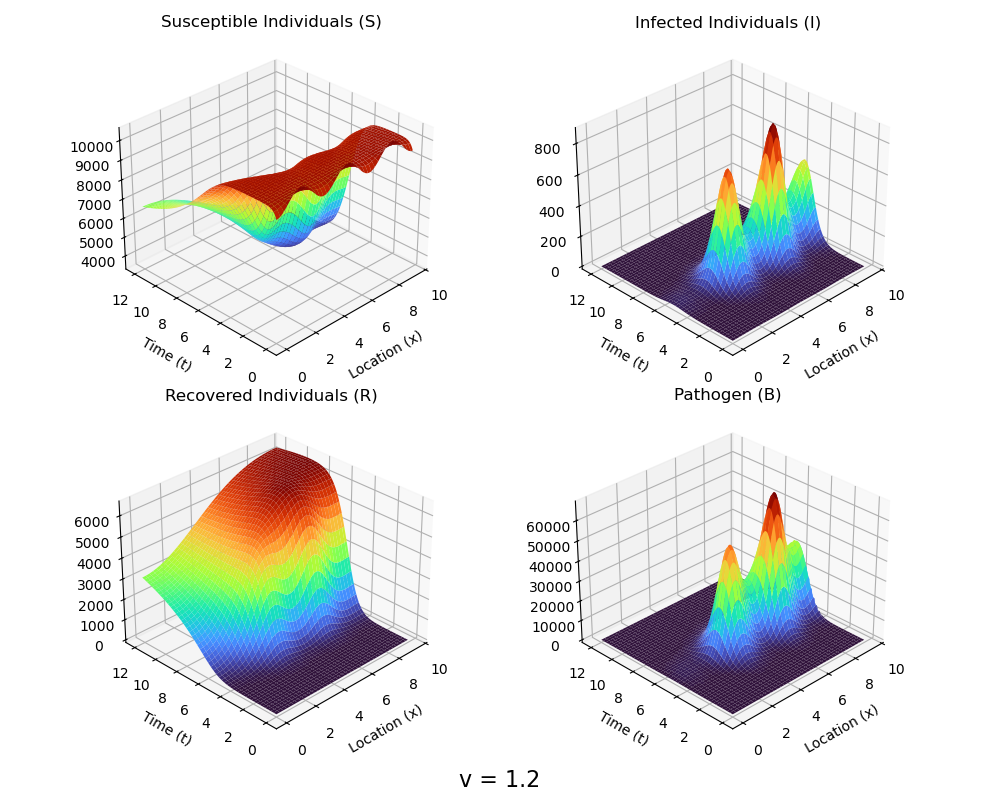
\includegraphics[width=0.6\textwidth]{Images/SpatialAccuracy.png}
\caption{Log-log Plot of Convergence}
\label{fig:loglogplot}
\end{figure}
\quad Figure \ref{fig:loglogplot} displays the log-log plot of the spatial step size versus the numerical error. The calculated error strictly follows the reference line of slope 2, yielding a computed order of accuracy of $k = 1.9119$. To achieve the exact halving of the spatial step size ($h$, $h/2$, $h/4$) required for this extrapolation, we follow a basic formula to calculate the required number of nodes. For a grid with $N_x$ nodes, there are $N_x - 1$ spatial intervals. To halve the step size, we must double the number of intervals, resulting in a new grid size of $2(N_x - 1) + 1 = 2N_x - 1$. For our spatial analysis, we initialize the base grid with $N_{x,1} = 200$ nodes. Subsequently, we calculate the refined grids as $N_{x,2} = 2(200) - 1 = 399$ nodes, and $N_{x,3} = 2(399) - 1 = 797$ nodes. 

\quad Our numerical result for the spatial accuracy analysis is as expected. Our usage of second order forward/backward difference approximation for the boundary conditions as well as the usage of second order central difference for first and second derivative for the interior nodes are the theoretical backbone for our numerical result. As established in our stability analysis, the temporal step size is strictly bounded by the spatial step size via the CFL condition ($\frac{\Delta t }{ \Delta x^2}$). Consequently, halving the spatial step size requires quartering the temporal step size to maintain stability, resulting in an eight-fold increase in total computational cost for each level of refinement.



% !TEX root = main.tex
\section{Discussion}
\subsection{Impact of Advection on Spatial-Temporal Dynamics}
\begin{figure}[H]
    \centering
    \begin{subfigure}[b]{0.48\textwidth}
        \centering
        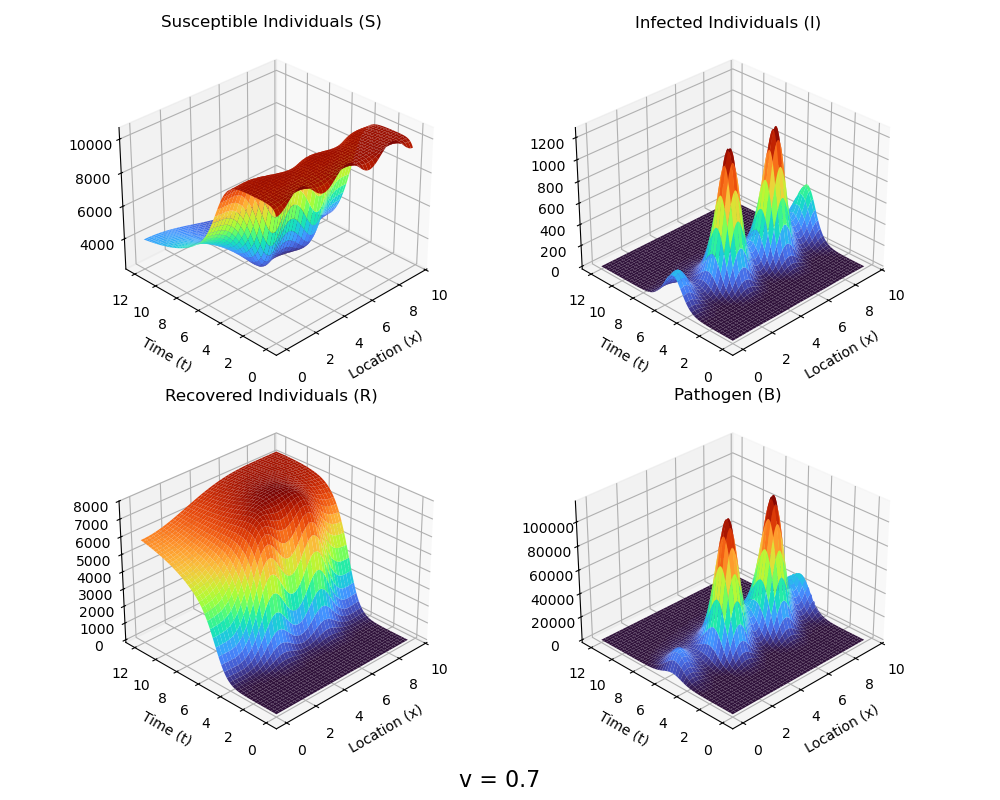
\includegraphics[width=\textwidth]{Images/v0.png}
        \caption{$v = 0.0$}
        \label{fig:v0}
    \end{subfigure}
    \hfill
    \begin{subfigure}[b]{0.48\textwidth}
        \centering
        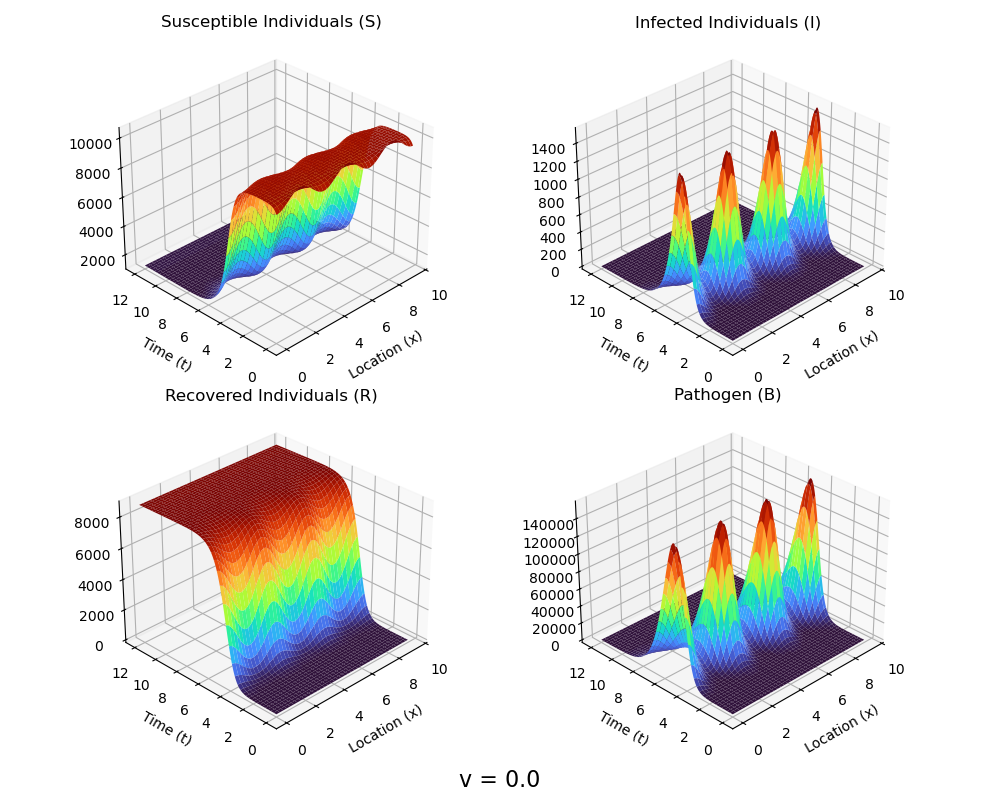
\includegraphics[width=\textwidth]{Images/v0.1.png}
        \caption{$v = 0.1$}
        \label{fig:v0.1}
    \end{subfigure}
    \caption{}
    \label{fig:advection_slow}
    %\caption{Spatiotemporal evolution of the cholera model under stagnant ($v=0.0$) and slow-flowing ($v=0.1$) conditions.}
    
\end{figure}
For Figure \ref{fig:advection_slow} we see the result off two values of $v= 0, \, 0.1$ tested in our simulation. These values were chosen to simulate stagnant water flow and slow-flowing water in the river respectively. As we can see from the 3-D graphs, they both share similar traits. For example, the spatial grid sees vary little variation as $x$ moves from $0$ to $3\pi$ towards the beginning and the end of the temporal domain. We can also see waves in the susceptible graphs as well as obvious peaks and valleys in the graphs midway through the simulated year, $t = 6$. Spatially, these occur along 4 different locations along the river. The most notable difference is in the graphs between both graphs of the pathogen at $v=0$ and $v=0.1$. The susceptible graph and infected graphs are inversely related. The graph of susceptible individuals drops significantly as time progresses while recovered individuals increases significantly as time increases. We expect these basic results as they serve as a control for the simulation. 




\begin{figure}[H]
    \centering
    \begin{subfigure}[b]{0.48\textwidth}
        \centering
        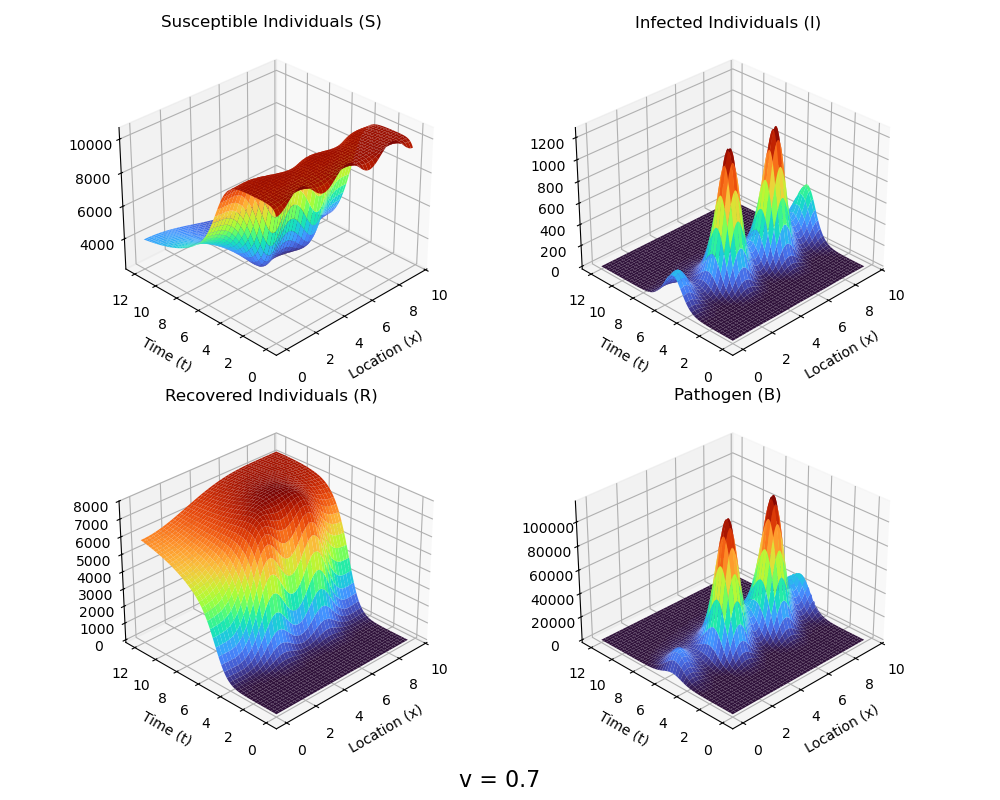
\includegraphics[width=\textwidth]{Images/v.7.png}
        \caption{$v = 0.7$}
        \label{fig:v.7}
    \end{subfigure}
    \hfill
    \begin{subfigure}[b]{0.48\textwidth}
        \centering
        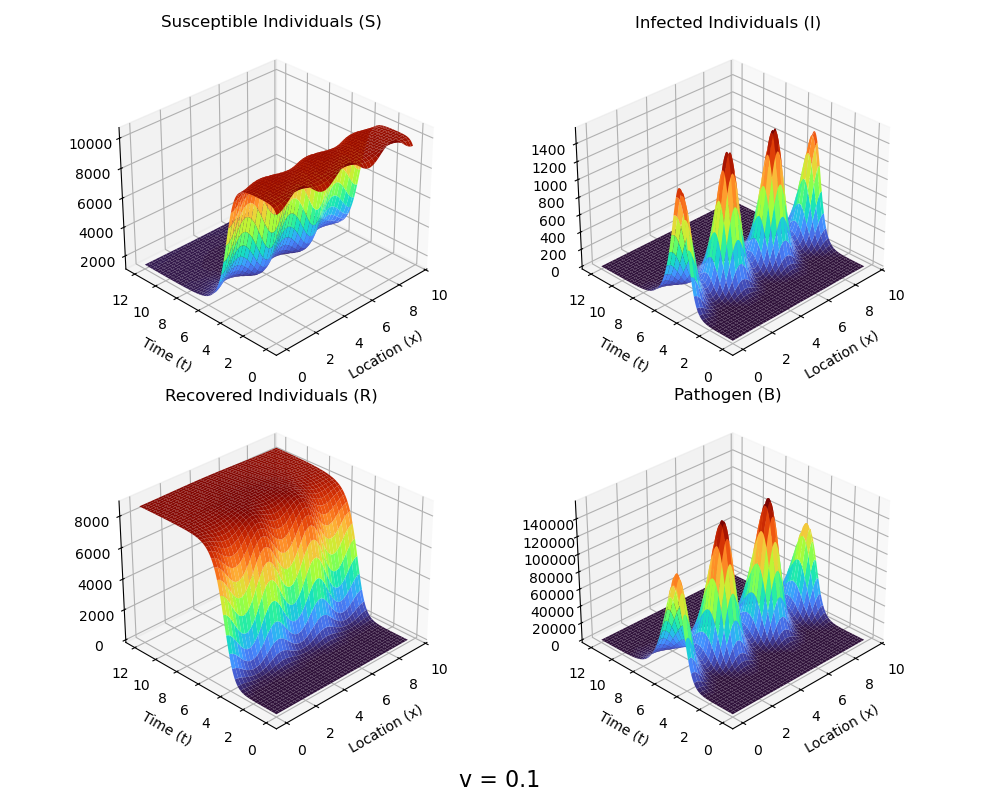
\includegraphics[width=\textwidth]{Images/v1.2.png}
        \caption{$v = 1.2$}
        \label{fig:v1.2}
    \end{subfigure}
    \caption{}
    %\caption{Spatiotemporal evolution under moderate ($v=0.7$) and fast-flowing ($v=1.2$) conditions. The advection dominates the diffusion, sweeping the pathogen downstream and causing it to accumulate against the zero-flux boundary at $x = 3\pi$.}
    \label{fig:advection_fast}
\end{figure}
\quad For Figure~\ref{fig:advection_fast}, we see the results of two higher advection values, $v = 0.7$ and $v = 1.2$, which were chosen to simulate moderate and fast-flowing river conditions, respectively. In these scenarios, advection heavily dominates diffusion. The river's current sweeps the pathogen downstream, causing a severe accumulation against the zero-flux boundary at $x = 3\pi$. Naturally as we see the concentration of the pathogen move downstream as time increases it follows that our other components follow suit. Across all subplots in Figure~\ref{fig:v.7} and Figure~\ref{fig:v1.2}, this downstream shift becomes highly pronounced. These graphical results help emphasize the importance of including the aquatic reservoir in the model (\cite{codeco2001endemic}).

\quad Comparing these faster advection rates to the slower speeds, the macroscopic effects of downstream transport become clear. As $v$ increases from $0$ to $1.2$, the rapid river flow, combined with spatial heterogeneity, creates a visible flattening effect on the upstream pathogen peaks. Biologically, the bacteria are washed away from their initial hotspots faster than they can locally reproduce. Consequently, the overall disease burden shifts toward the end of the river. This dynamic explains the spatial distribution of the human populations as time progresses. Therefore susceptible individuals are depleted much more rapidly at the downstream boundary, which in turn creates a highly concentrated, localized spike of recovered individuals in that same area.

%As we can see from the 3-D graphs, they both share similar traits. For example, the spatial grid sees vary little variation as $x$ moves from $0$ to $3\pi$ towards the beginning and the end of the temporal domain. We can also see waves in the susceptible graphs as well as obvious peaks and valleys in the graphs midway through the simulated year, $t = 6$. Spatially, these occur along 4 different locations along the river. The most notable difference is in the graphs between both graphs of the pathogen at $v=0$ and $v=0.1$. The susceptible graph and infected graphs are inversely related. The graph of susceptible individuals drops significantly as time progresses while recovered individuals increases significantly as time increases. We expect these basic results as they serve as a control for the simulation. 
\newpage %----------------------------------------------
% !TEX root = main.tex
\section{Conclusion}
To summarize we first started with a reaction diffusion model for waterborne infection of Cholera. Since our model consists of several PDEs we turn to a numerical approach for a solution. Using second order central finite difference formula for the spatial derivative we derived a numerical scheme for our model. Furthermore, we ensured the no-flux boundary conditions were derived using second order forward/backward difference formulas to maintain a theoretical accuracy of $\mathcal{O}(\Delta x^2)$. We presented our initial conditions and biological parameters based on prior academic research in this related field. As we noted in earlier sections, the proven numerical stability and accuracy ensure the physical validity and reliability of our simulated epidemic dynamics. 

\quad A natural direction for future research using this model would be a more in-depth analysis of the biological impacts of the parameters used. While our current results provide valuable insights, exploring a wider parameter space is required to fully understand the disease dynamics. For example, we primarily simulated different choices of the pathogen's advection rate, $v$, which represents the speed of the river flow. During our simulations, all other parameters remained unchanged, including our initial conditions. Modifying other parameters, such as the pathogen death rate, the diffusion rate, or utilizing a closed SIRB model with a fixed human population, would all be excellent areas of focus for future research. Ultimately, our findings indicate a significant increase in the downstream spread and localized accumulation of the pathogen as the river flow speed increases.

\quad You can find my GitHub repo \href{https://github.com/ethanreyes78/phd-rd-solver}{HERE}.

\newpage %------------------------------------------------------------

\printbibliography

\end{document}